\documentclass[a4paper,12pt]{article}

\usepackage[T1]{fontenc}
\usepackage{times}
\usepackage[swedish,english]{babel}
\usepackage[utf8]{inputenc}
\usepackage{dtklogos}
\usepackage{wallpaper}
\usepackage[absolute]{textpos}
\usepackage[top=2cm, bottom=2.5cm, left=3cm, right=3cm]{geometry}
\usepackage{appendix}
\usepackage[nottoc]{tocbibind}
%\usepackage{setspace}

\setcounter{secnumdepth}{3}
\setcounter{tocdepth}{3}

\usepackage{sectsty}
\sectionfont{\fontsize{14}{15}\selectfont}
\subsectionfont{\fontsize{12}{15}\selectfont}
\subsubsectionfont{\fontsize{12}{15}\selectfont}

\usepackage{csquotes} % Used to handle citations
\renewcommand{\thetable}{\arabic{section}.\arabic{table}}  
\renewcommand{\thefigure}{\arabic{section}.\arabic{figure}}

%----------------------------------------------------------------------------------------
%	
%----------------------------------------------------------------------------------------
\newsavebox{\mybox}
\newlength{\mydepth}
\newlength{\myheight}

\newenvironment{sidebar}%
{\begin{lrbox}{\mybox}\begin{minipage}{\textwidth}}%
{\end{minipage}\end{lrbox}%
 \settodepth{\mydepth}{\usebox{\mybox}}%
 \settoheight{\myheight}{\usebox{\mybox}}%
 \addtolength{\myheight}{\mydepth}%
 \noindent\makebox[0pt]{\hspace{-20pt}\rule[-\mydepth]{1pt}{\myheight}}%
 \usebox{\mybox}}

%----------------------------------------------------------------------------------------
%	Title section
%----------------------------------------------------------------------------------------
\newcommand\BackgroundPic{
    \put(-2,-3){
    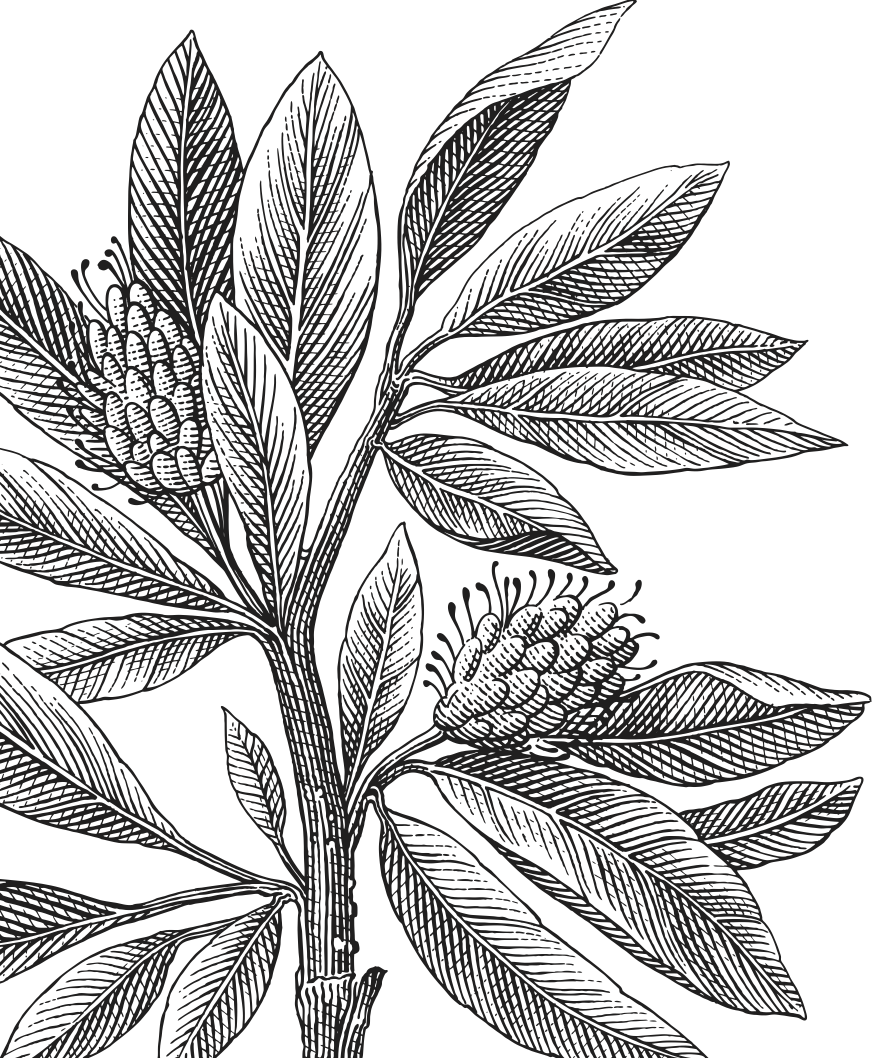
\includegraphics[keepaspectratio,scale=0.3]{img/lnu_etch.png} % Background picture
    }
}
\newcommand\BackgroundPicLogo{
    \put(30,740){
    
\includegraphics[keepaspectratio,scale=0.10]{img/logo.png} % Logo in upper left corner
    }
}

\title{	
\vspace{-8cm}
\begin{sidebar}
    \vspace{10cm}
    \normalfont \normalsize
    \Huge Assignment 1: Jodel Alert \\
    \vspace{-1.3cm}
\end{sidebar}
\vspace{3cm}
\begin{flushleft}
    \huge Software Engineering - Design\\ 
    \it \LARGE - 2DV603
\end{flushleft}
\null
\vfill
\begin{textblock}{6}(10,12)
\begin{flushright}
\begin{minipage}{\textwidth}
\begin{flushleft} \large
\emph{Name:} Patrik Hermansson\\ % Author
\emph{Email:} ph222md@student.lnu.se\\
\emph{Name:} Michael Wagnberg\\ % Author
\emph{Email:} mw222uu@student.lnu.se\\
\emph{Name:} Benjamin Svärd\\ % Author
\emph{Email:} bs222et@student.lnu.se\\
\emph{Name:} Christofer Nguyen\\ % Author
\emph{Email:} cn222hn@student.lnu.se\\
\emph{Name:} Jonathan Walkden\\ % Author
\emph{Email:} jw222qi@student.lnu.se\\
\end{flushleft}
\end{minipage}
\end{flushright}
\end{textblock}
}

\date{} 
\newpage
\begin{document}
\pagenumbering{gobble}
\newgeometry{left=5cm}
\AddToShipoutPicture*{\BackgroundPic}
\AddToShipoutPicture*{\BackgroundPicLogo}
\maketitle
\restoregeometry
\selectlanguage{english}
\pagenumbering{gobble}
\newpage
\tableofcontents % Table of contents
\pagenumbering{arabic}
\newpage
\section{Domain Analysis Document}
\subsection{Introduction}
Words from our customer:
Jodel is a new anonymous social app targeting students
and campus life. Some questions and comments posted
there are specifically related to things that the Student
Union deal with, i.e. questions about accommodation,
what rules apply when writing an exam, if you need a
student ID to get into the pubs etc. We’d love to
comment on such questions, but they are far between
and we haven’t got time to monitor the feeds so if
possible it would be great to have functionality that
could tap into the Jodel API and send e-mail alerts if
relevant keywords show up; similar to Google Alerts or
Meltwater.
\\
We are supposed to create an application that will listen for keywords entered in posts in the Jodel application, and when keyword found an email will be generated and sent to Linnéstudenterna. They will then know that a post has been made that regards Linnéstudenterna and can act upon.
\section{Assignment 1}
Requirements
\\\\
\section{Problem}

\section{Background information}

\section{Environment and system models}

\begin{figure}[!h]
	\centering
	
\includegraphics[height=6cm]{img/jodel.png}
	\caption{Jodel logo}
	\label{Cisco routing}
\end{figure}
\section{Functional requirements}
\begin{enumerate}
	\item When a keyword is used in a Jodel post, Linnestudenterna will receive a mail
	\item Keywords should be able to be removed
	\item Keywords should be able to be added
	\item Keywords should be able to be changed
	\item Added keywords saved between sessions (i.e saved on local host if you restart the app)
	\item Recipient email should be able to be removed
	\item Recipient email should be able to be added
	\item Recipient email should be able to be changed
\end{enumerate}
\section{Non-functional requirements}
\begin{enumerate}
	\item App will continuously scan Jodel traffic
	\item When a keyword has been found, email should be sent within 2 seconds
\end{enumerate}

\end{document}